%----------------------------------------------------------------------------------------
%	PACKAGES AND OTHER DOCUMENT CONFIGURATIONS
%----------------------------------------------------------------------------------------

\documentclass[twoside,twocolumn]{article}
%________My packages Begin_____________________________________

\usepackage{graphicx} % for figures
\usepackage{float}% necessary "begin{figure}[H] to Place the float at precisely the location in the LaTeX code.
%=--------------------Francais------------
\usepackage[french]{babel} %Texte en fran�ais
\usepackage{lmodern}
\usepackage[utf8]{inputenc}
%-------------------------------

\usepackage[normalem]{ulem}
\usepackage{mathtools}
\usepackage{fourier}
\usepackage{enumitem}
\usepackage[skins,theorems]{tcolorbox}% for boxing and coloring equations
\usepackage{amsmath,amsthm,amssymb}
%-----
\apptocmd{\thebibliography}{\csname phantomsection\endcsname\addcontentsline{toc}{chapter}{\bibname}}{}{}
\usepackage[toc,page]{appendix}
\usepackage[nottoc]{tocbibind}
%\usepackage{lmodern}
%\renewcommand{\familydefault}{lmodern}
\usepackage{stfloats}
%________My packages End _________________________

%\usepackage[sc]{mathpazo} % Use the Palatino font

\usepackage[T1]{fontenc} % Use 8-bit encoding that has 256 glyphs
\linespread{1.05} % Line spacing - Palatino needs more space between lines
\usepackage{microtype} % Slightly tweak font spacing for aesthetics

%\usepackage[english]{babel} % Language hyphenation and typographical rules

\usepackage[hmarginratio=1:1,top=28mm,columnsep=30pt]{geometry} % Document margins
\usepackage[hang, small,labelfont=bf,up,textfont=it,up]{caption} % Custom captions under/above floats in tables or figures
\usepackage{booktabs} % Horizontal rules in tables

\usepackage{lettrine} % The lettrine is the first enlarged letter at the beginning of the text

\usepackage{enumitem} % Customized lists
\setlist[itemize]{noitemsep} % Make itemize lists more compact

\usepackage{abstract} % Allows abstract customization
\renewcommand{\abstractnamefont}{\normalfont\bfseries} % Set the "Abstract" text to bold
\renewcommand{\abstracttextfont}{\normalfont\small\itshape} % Set the abstract itself to small italic text

\usepackage{titlesec} % Allows customization of titles
\renewcommand\thesection{\Roman{section}} % Roman numerals for the sections
\renewcommand\thesubsection{\roman{subsection}} % roman numerals for subsections
\titleformat{\section}[block]{\large\scshape\centering}{\thesection.}{1em}{} % Change the look of the section titles
\titleformat{\subsection}[block]{\large}{\thesubsection.}{1em}{} % Change the look of the section titles

\usepackage{fancyhdr} % Headers and footers
\pagestyle{fancy} % All pages have headers and footers
\fancyhead{} % Blank out the default header
\fancyfoot{} % Blank out the default footer
\fancyhead[C]{Identification et Filtrage (IDFIL) : Travaux Pratiques n° 1 $\bullet$ Ecole Centrale de Nantes $\bullet$} % Custom header text
\fancyfoot[RO,LE]{\thepage} % Custom footer text

\usepackage{titling} % Customizing the title section

\usepackage[hidelinks]{hyperref} % For hyperlinks in the PDF

%----------------------------------------------------------------------------------------
%	TITLE SECTION
%----------------------------------------------------------------------------------------

\setlength{\droptitle}{-4\baselineskip} % Move the title up

\pretitle{\begin{center}\Huge\bfseries} % Article title formatting
\posttitle{\end{center}} % Article title closing formatting
\title{Identification et Filtrage (IDFIL)  Travaux Pratiques n° 1} % Article title

\author{%
\noindent\rule{6cm}{1pt} \\ \\
\LARGE
\textsc{Housseyne NADOUR}\\[1ex] % Your name
\normalsize Master ARIA, ASI \\ % Your institution
\\
\normalsize Sous direction de l'ensignant \\ % Your institution
\LARGE
\textsc{Saïd Moussaoui}\\[1ex] % Your name
\noindent\rule{6cm}{1pt} \\ \\
}
\date{\today} 

%================Matlab
%-----------------------------------------------
\usepackage[T1]{fontenc}
\usepackage{bigfoot} % to allow verbatim in footnote
\usepackage[numbered,framed]{matlab-prettifier}
\usepackage{filecontents}

\let\ph\mlplaceholder % shorter macro
\lstMakeShortInline"

\lstset{
  style              = Matlab-editor,
  basicstyle         = \mlttfamily,
  escapechar         = ",
  mlshowsectionrules = true,
}

\begin{filecontents*}{1.m}
%% L'ordre de chaque filtre:
%% Butterworth:
[nc_b, wnc_b]= buttord(2*pi*fp,2*pi*fa,Ap,Aa,'s'); % en analogique
%% Chabyshev de type 1:
[nc_c1, wnc_c1]= cheb1ord(2*pi*fp,2*pi*fa,Ap,Aa,'s'); % en analogique
%% Chabyshev de type 2:
[nc_c2, wnc_c2]= cheb2ord(2*pi*fp,2*pi*fa,Ap,Aa,'s'); % en analogique
%% Chabyshev de ellipe:
[nc_el, wnc_el]= ellipord(2*pi*fp,2*pi*fa,Ap,Aa,'s'); % en analogique
\end{filecontents*}
\begin{filecontents*}{2.m}
%% B) Les coefficients de chaque filtre:
% Butterworth:
[numc_b, denc_b] = butter(nc_b,wnc_b,'low','s');% en analogique
% Chabyshev de type 1:
[numc_c1, denc_c1] = cheby1(nc_c1,Ap,wnc_c1,'low','s');% en analogique
% Chabyshev de type 2:
[numc_c2, denc_c2] = cheby2(nc_c2,Aa,wnc_c2,'low','s');% en analogique
% Chabyshev de ellipe:
[numc_el, denc_el] = ellip(nc_el,Ap,Aa,wnc_el,'low','s');% en analogique
H_ellip = tf(numc_el, denc_el);
\end{filecontents*}

\begin{filecontents*}{3.m}
%% La reponse frequentielle de chaque filtre analogique:
 f = linspace(fmin,fmax,1000);
 Hc_b = freqs(numc_b,denc_b,2*pi*f);  
 Hc_c1 = freqs(numc_c1,denc_c1,2*pi*f);  
 Hc_c2 = freqs(numc_c2,denc_c2,2*pi*f); 
 Hc_el = freqs(numc_el,denc_el,2*pi*f); 
 
\end{filecontents*}
\begin{filecontents*}{30.m}
H_ellip = tf(numc_el, denc_el);
margin(H_ellip);
\end{filecontents*}

\begin{filecontents*}{4.m}
graph = plot(f,20*log10(abs(Hc_b)),f,20*log10(abs(Hc_c1)),f,20*log10(abs(Hc_c2)),f,20*log10(abs(Hc_el)));
 legend(graph,'Butterworth','Chabyshev de type 1','Chabyshev de type 2','Cauer')
\end{filecontents*}

\begin{filecontents*}{5.m}
%% Filter and listen:
Filtred_Signal_ButterWorth = lsim(tf(numc_b,denc_b),sig,t);
soundsc(Filtred_Signal_ButterWorth, fe);
Filtred_Signal_Cheb1 = lsim(tf(numc_c1,denc_c1),sig,t);
soundsc(Filtred_Signal_Cheb1, fe);
Filtred_Signal_Cheb2 = lsim(tf(numc_c2,denc_c2),sig,t);
soundsc(Filtred_Signal_Cheb2, fe);
Filtred_Signal_Cauer = lsim(tf(numc_el,denc_el),sig,t);
soundsc(Filtred_Signal_Cauer, fe);

\end{filecontents*}

\begin{filecontents*}{6.m}
figure(2);
subplot(2,2,1); plot(t,Filtered_Signal_ButterWorth);title('ButterWorth');
subplot(2,2,2); plot(t,Filtered_Signal_Cheb1);title('Cheb1');
subplot(2,2,3); plot(t,Filtered_Signal_Cheb2);title('Cheb2');
subplot(2,2,4); plot(t,Filtered_Signal_Cauer);title('Cauer');

 legend(graph,'Butterworth','Chabyshev de type 1','Chabyshev de type 2','Cauer')
\end{filecontents*}

\begin{filecontents*}{7.m}
%% Chabyshev de type 2:
Df = 10;
fc_b = 340; 
fc_h=360; 
% Df = 5;
% fc_b = 345; 
% fc_h=355; 

fp_b = fc_b - Df/2;
fp_h = fc_h - Df/2;
fa_b = fc_b + Df/2;
fa_h = fc_h + Df/2;
Wp = 2*[fa_b fp_h]/fe; % IN
Ws = 2*[fp_b fa_h]/fe; % EX
Ap=1; Aa=40;
%% A) Filtrage Coup-Bande analogique
%% L'ordre de chaque filtre:
[nd_c2, wnd_c2]= cheb2ord(Wp,Ws,Ap,Aa) ;
%% B) Les coefficient de chaque filtre:
[numd_c2, dend_c2] = cheby2(nd_c2,Aa,wnd_c2,'stop');
%  
%% C) Les reponses frequentielles;
 figure(2)
 f = linspace(fmin,fmax,1000);
 Hd_c2 = freqz(numd_c2,dend_c2,f,fe); plot(f,20*log10(abs(Hd_c2)));
\end{filecontents*}

\begin{filecontents*}{8.m}
%% D1) Tracer sur la meme figure l allure temporelle et le spectre d amplitude de lagamme filtree
 figure(3)
 Cheb2 = filter(numd_c2,dend_c2,sig);
 plot(t,Cheb2);title('Cheb2');
 %% D2) Le spectre d'amplitude de la gamme filtree
figure(4)
ffc = [0:length(Cheb2)-1]*(fe/length(Cheb2));
fmin = 100; fmax = 600; ymax = 0.6;
Sfc = fft(Cheb2)/fe;  plot(ffc, abs(Sfc));  axis([fmin fmax 0 ymax]); hold on;
soundsc(Cheb2, fe)
\end{filecontents*}
\begin{filecontents*}{9.m}
%% Filtre RIF de longueur minimale (fenetre de Kaiser) :
%% A) L'ordre de chaque filtre:
 ep = 1-10^(-Ap/20); da = 10^(-Aa/20);
 [n,wc,beta] = kaiserord([fp_b fa_b fp_h fa_h],[1 0 1],[ep da ep],fe);
 %% B) La fenetre:
 h = fir1(n,wc,'stop',kaiser(n+1,0.5),'noscale') ;
 %% D1) La reponse frequentielle du filtre de Kaiser:
%f = linspace(fmin,fmax,1000);
[HK,f] = freqz(h,1,f,fe);
figure(5)
plot(f,20*log10(abs(HK))); axis([fmin fmax -70 10]);

%% C) Tracer l allure temporelle  de l agamme filtree
 figure(6)
 Filtered_Kaiser = filter(h,1,sig);
 plot(t,Filtered_Kaiser);title('Filtered_Kaiser');
 %Analyse frequentielle d'un signal apres filtrage:
    figure(6)
    ffc = [0:length(Filtered_Kaiser)-1]*(fe/length(Filtered_Kaiser));
    fmin = 250; fmax = 600; ymax = 0.6;
    Sfc = fft(Filtered_Kaiser)/fe;  plot(ffc, abs(Sfc));  axis([fmin fmax 0 ymax]); hold on;  
    %% Listen:
   soundsc(Filtered_Kaiser, fe)
\end{filecontents*}

%================================================

\renewcommand{\maketitlehookd}{%
\begin{abstract}
\large
L'objective de ce TP est de mettre en pratique, les différents techniques de filtrage, et comparer entre eux, les filtres á synthétiser sont des filtre Analogiques, filtres RII, et des filtres RIF, Ce travaille est composé de deux parties, dans chaque partie on analyse ces différent types de
filtres.
\end{abstract}
}


%----------------------------------------------------------------------------------------

\begin{document}

% Print the title
\maketitle
\
%----------------------------------------------------------------------------------------
%	ARTICLE CONTENTS
%----------------------------------------------------------------------------------------
\tableofcontents

\section{Le signale á filtrer:}

Les filtres á synthétiser seront appliqués sur un signal de durée de $8s$, composé successivement de 8 signales sinusoïdales de fréquences différentes et de même durée ($1s$) .\\
La fréquence d'échantillonnage a été choisi de telle façon de respecter \underline {le théorème de Schannone} qui consiste á choisir la fréquence d'échantillonnage deux fois plus grande que la plus grande fréquence que le signale comporte pour extraire toute les informations utiles dans ce signale, dans notre cas la plus grande fréquence est: $523$ Hz, tant que la fréquence d'échantillonnage $f_e = 8192$, d'où le théorème de Shcannone est respecté.

\section{Filtrage pas-bas analogique}
\subsection{L'ordre de chaque filtre}
Le script du Matlab pour calculer l'ordre de chaque filtre:

\label{matlab}
\lstinputlisting[caption = {Le script du Matlab pour calculer l'ordre de chaque filtre}]{1.m}

\begin{tabular}{l|r}
Type du filtre & L'ordre du filtre \\
Butterworth & 20 \\
Chabyshev de type 1 & 8\\
Chabyshev de type 2 & 8\\
Cauer &  5\\
\end{tabular}
\\
\\
\underline{Remarque:}\\

Il est claire que la méthode de Butterworth a le plus grand ordre$n$, par contre le filtre de Cauer a le plus petit ordre, et les deux types de chabychev ont le même ordre entre les filtre de Butterworth et Cauer.
 On peut dire alors que le filtre de Cauer est le moins couteux parmi les autres filtres analogiques que signifie que ce filtre est simple a synthétiser, et n'exige pas beaucoup de calcul et beaucoup de temps pour filtrer le signal.

Le script suivant a pour objective de calculer les coefficients de dénominateur et numérateur de chaque filtre:

\label{matlab}
\lstinputlisting[caption = {Le script du Matlab pour calculer l'ordre de chaque filtre}]{2.m}

Par exemple le filtre Cauer est de la forme suivante:\\ 

$H_{ellip} = \frac{94.79 s^4 + 6.36e-12 s^3 + 1.978e09 s^2 - 3.073e-06 s + 9.42e15}{  s^5 + 1319 s^4 + 8.828e06 s^3 + 8.501e09 s^2 + 1.823e13 s + 9.42e15}$\\

la fonction de transfert de ce filtre est plus compact que celles des autres filtres.

\subsection{les réponses fréquentielles en amplitude des quatre filtres}

le script suivant permet d'obtenir les valeurs numériques de chaque fonctions de transfert (chaque filtre) pour chaque valeur de fréquence f:


\label{matlab}
\lstinputlisting[caption = {Le script du Matlab pour calculer la réponse de chaque filtre}]{3.m}

	On peut utiliser la fonction $margin$ ou la fonction $bode$  pour tracer les réponses en amplitude  en phase :
	\label{matlab}
\lstinputlisting[caption = {réponse fréquentielle du filtre de Cauer}]{30.m}
	Mais avec ce scripte, les réponses sont dessinées en fonction de la pulsation au lieu de la fréquence ($\omega = 2.\pi.f$).\\
	pour obtenir les réponses en fréquence on utilise  le script suivant:
	
	\label{matlab}
\lstinputlisting[caption = {Le script  pour tracer les réponses fréquentielles}]{4.m}

Les réponses sont illustrées sur la figure suivante:
\begin{figure}[H]
\centering
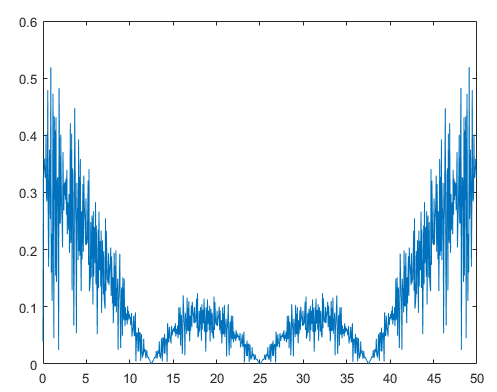
\includegraphics[width=0.5\textwidth]{Images/3.png}
\caption{ la réponse fréquentielle de chaque filtre}
\end{figure}

\underline{Remarque:}\\

Le graphe montre des caractéristiques commune et autre différentes entre les quatre filtres synthétisés: 
\begin{itemize}
\item
Tout les filtre synthétisé rejettent tous les signaux de fréquence supérieur á la fréquence de coupure désirée $fc = 420$
\item
La fréquence de coupure reélle n'est pas confondue á celle désirée (l'idéelle est 420 Hz), en effet les courbes montrent que la fréquence de coupure réelle est 360 Hz, dans notre ça ne pose pas le problem de rejeter des signaux utiles parce que le signal á filtrer comporte des fréquences espacées entre elles.
\item
La caractéristique en amplitude du filtre Butterworh est très plate dans la bande passante, et lisse dans bande coupée, et ça revient á l'ordre élevé du filtre.
Par contre les autre filtres présentent de oscillations dans la bande passante á cause de l'ordre réduit de chaque filtre.

\item
Les deux filtres Chebytchev type 1 et Cauer sont plus proches du filtre idéal que les filtres Butterworth et Chebytchev de type 2, parce qu'ils ont une coupure \underline{extrêmement raide}.
\end{itemize}

\subsection{Filtrage du signal audio}

\label{matlab}
\lstinputlisting[caption = {Le script du Matlab pour filtrer la gamme, et écoûter les gammes filtrées}]{5.m}

Les trois dernier notes ont été partialement rejetées, en plus la note $Sol$ (qui est considérés comme une information utile dans la bande passante) a été influencée par le filtre, malgré qu'on ne peut jamais synthétiser un filtre idéal, mais pour notre signale ou les fréquence des notes sont espacées, on peut modifier les paramètres du filtre(la bande passantes et les amplitudes) pour rejeter parfaitement les trois dernières note sans influencer aucune note utile.\\
 En faite, les paramètres suivants satisfont l'objective désiré :\\
$f_c = 425\quad Hz$  \quad au lieu  \quad $f_c = 420\quad Hz$ \\
$\Delta f = 60\quad Hz$ \quad au lieu \quad $\Delta f = 100\quad Hz$ \\
$A_a = 50$ \quad au lieu \quad $A_a = 40$\\
	Les nouveaux réponses fréquentielles:
\begin{figure}[H]
\centering
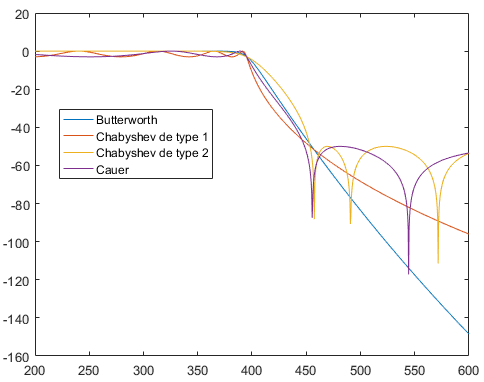
\includegraphics[width=0.5\textwidth]{Images/4.png}
\caption{ la réponse fréquentielle de chaque filtre après l'amélioration}
\end{figure}
Touts les filtres rejettent d'une manière presque parfaite les trois dernières notes et sans affecter la note $Sol$.\\
	Mais cet avantage est payé par un augmentation dans les ordres des filtres:\\
	\\
	\begin{tabular}{l|r}
Type du filtre & L'ordre du filtre \\
Butterworth & 41 \\
Chabyshev de type 1 & 12\\
Chabyshev de type 2 & 12\\
Cauer &  6\\
\end{tabular}
\\
\\
\underline{Remarque:}\\
La méthode de Cauer montre une caractéristique inter issante, son ordre n'a augmenté que de $20\%$, tant  
que celui de Butterworth a augmentés de plus que $100\%$, et l'ordre de Chabyshev de type 1 et 2 ont un augmentation de  $50\%$.\\
Cet résultat montre que le filtre de Cauer est le meilleur choix.

\subsection{Le graphe de l'allure de la gamme filtrée dans le domaine temporel et fréquentiel}
premièrement, on tracer l'allure du signale filtré en utilisant les paramétrés données dans la question. puis on trace l'allure en utilisant les paramètres proposés. 
\label{matlab}
\lstinputlisting[caption = {Le script du Matlab pour la gamme filtrées dans le domaine temporel}]{6.m}
\subsubsection{L'allure dans le domaine temporel}
\begin{figure}[H]
\centering
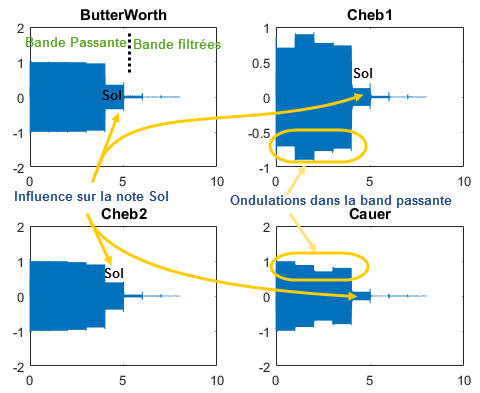
\includegraphics[width=0.5\textwidth]{Images/5.png}
\caption{ L'allure dans le domaine temporel de la gamme filtrée}
\end{figure}

\underline{Remarque:}
Ce graphe confirme les remarques qu'on a constaté précédemment:
\begin{itemize}
\item
Les notes á filtrer ($La$ $Si$ $Do$) ont été rejetés mieux par le filtre Cauer et Chebychev 1 que Butterworth et Chebychev 2.
\item
La note $Sol$ a été influencée par le filtrage, On ne va plus remarquer cette inconvénient   après l'amélioration des paramètres du filtre (Voire le graphe suivant).
\item 
On remarque des ondulation dans la bande passant pour le filtre de Chebycheve type 1 et le filtre de Cauer, c'est le coût d'avoir une coupure raide (bande transitoire très courte), cette remarque est confirmée par la réponse fréquentielle qui montre des ondulation dans la bande passante.
Par contre les deux filtres de Butterworth et Chebychev type 2, ne présentent pas cet inconvénient. surtout le filtre de Butterworth, c'est expliqué par la réponse fréquentielle qui montre une caractéristique en amplitude très plate dans la bande passante.
\item Les altérations du signal filtré dans la bande passante (les ondulations) signifie que le volume du son change dans la bande passante.

\end{itemize}
%\newpage
Si on utiliser les paramètres suivant :\\
 $f_c = 425\quad Hz$  \quad au lieu  \quad $f_c = 420\quad Hz$ \\
$\Delta f = 60\quad Hz$ \quad au lieu \quad $\Delta f = 100\quad Hz$ \\
$A_a = 50$ \quad au lieu \quad $A_a = 40$
 On trouve les résultats désirés.
 
\begin{figure}[H]
\centering
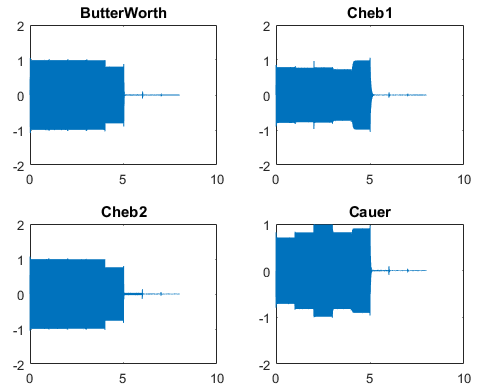
\includegraphics[width=0.5\textwidth]{Images/6.png}
\caption{ L'allure dans le domaine temporel de la gamme filtrée après l'amélioration des paramètres}
\end{figure}

\underline{Remarque:}
Le filtre de Butterworth montre des bonnes	 caractéristiques dans la bande passante et dans la bande coupée par rapport á les autres filtres , mais c'est payé par le coût de l'ordre de ce filtre ($n=40$).

\subsubsection{Le spectre d'amplitude de la gamme filtrée}

\begin{figure}[H]
\centering
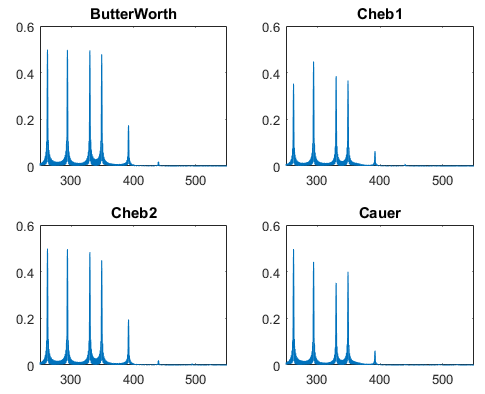
\includegraphics[width=0.5\textwidth]{Images/7.png}
\caption{ Le spectre de la gamme filtrée}
\end{figure}
Ce graphe confirme les points remarqués sur l'allure de la gamme filtrée dans le domaine temporel. 
En utilisant les paramètres proposés, on trouve des bons résultat dans les deux bandes, passantes et coupée.
\begin{figure}[H]
\centering
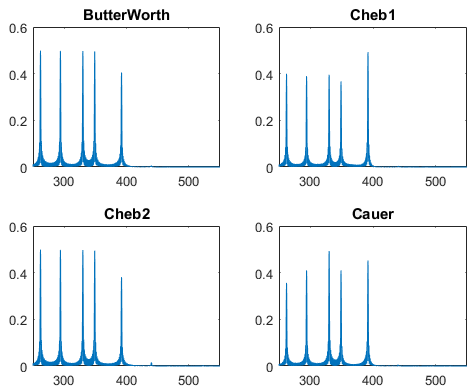
\includegraphics[width=0.5\textwidth]{Images/8.png}
\caption{ Le spectre de la gamme filtrée après l'amélioration des paramètres}
\end{figure}
\newpage
\subsection{Modification de le bande de transition}
le paramètre qui va se changer c'est:\\
 $\Delta f =20Hz$\\
On résume les résultats trouvés pour chaque filtre dans les graphes suivants :

\subsubsection{L'ordre de chaque filtre}

\begin{tabular}{l|r}
Type du filtre & L'ordre du filtre \\
Butterworth & 111 \\
Chabyshev de type 1 & 20\\
Chabyshev de type 2 & 20\\
Cauer &  7\\
\end{tabular}\\

\subsubsection{les réponses fréquentielles en amplitude des quatre filtres}
\begin{figure}[H]
\centering
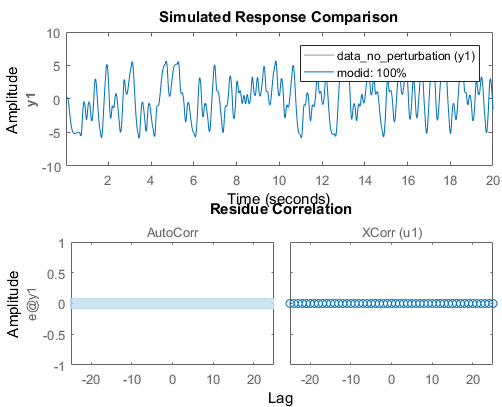
\includegraphics[width=0.5\textwidth]{Images/9.png}
\caption{ les réponses fréquentielles en amplitude des quatre filtres}
\end{figure}
\subsubsection{L'allure de la gamme filtrée dans le domaine temporel}
\begin{figure}[H]
\centering
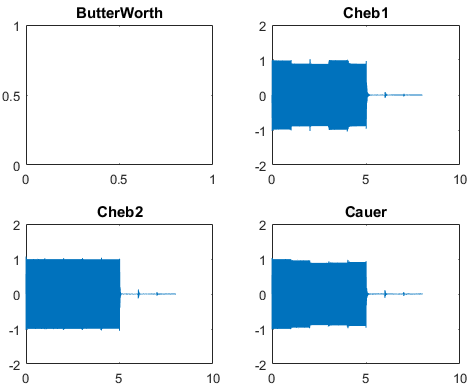
\includegraphics[width=0.5\textwidth]{Images/10.png}
\caption{ L'allure de la gamme filtrée dans le domaine temporel}
\end{figure}
\subsubsection{L'allure de la gamme filtrée dans le domaine fréquentiel}
\begin{figure}[H]
\centering
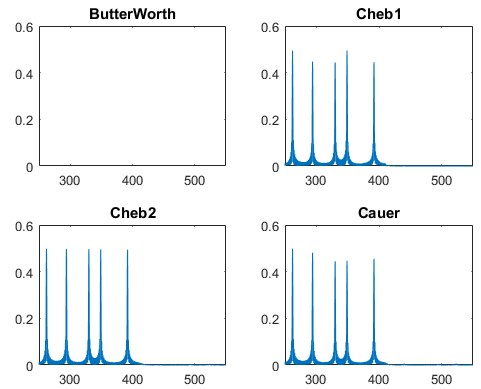
\includegraphics[width=0.5\textwidth]{Images/11.png}
\caption{ L'allure de la gamme filtrée dans le domaine fréquentiel}
\end{figure}

\underline{Remarque:}
On remarque des avantages et des inconvénients en modifiant la bande de transitoire:
\begin{itemize}

\item
L'ordre de chaque filtre a augmenté, surtout le filtre de Butterworth, qui a exigé un ordre de 111, et ça rend le filtre non applicable, et on peut voir que le matlab n'a pas pu dessiner les allures pour le filtre de Butterworth due au chut de calcul. par contre le filtre de Cauer reste toujours dans le cadre pratique due au son ordre qui est 7.

\item
Un bon filtrage de notes á rejeter dans la bande á coupée.

\item
Les ondulations dans la bandes passantes ont disparu, que signifie que le volume du son ne change pas dans la bande passante.
\item
Les filtres ont des coupure extremement raides (bande transitoire tres courte), et d'oú l'avantage suivant:

\item
Les signales outiles (comme la note Sol) ne ont pas été influencée par le filtrage.

\end{itemize}
\newpage
\newpage

\section{Elimination d’une note par filtrage coupe-bande}

\subsection{Filtre numérique coupe-bande de type Chebyshev 2}
Le script pour calculer le filtre :
\label{matlab}
\lstinputlisting[caption = {Le script pur calculer le Filtre numérique coupe-bande de type Chebyshev 2, et pour tracer la réponse fréquentielle}]{7.m}


\begin{figure}[H]
\centering
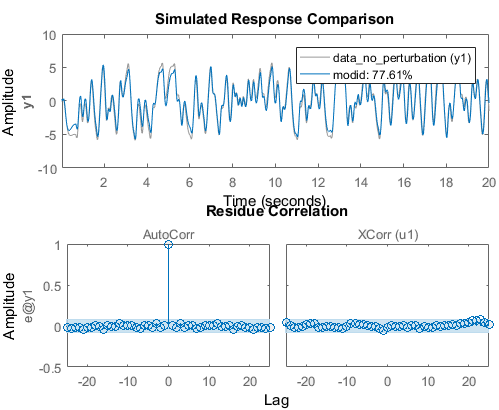
\includegraphics[width=0.5\textwidth]{Images/12.png}
\caption{ La réponse fréquentielle du filtre RII de type Chebychev 2}
\end{figure}
\begin{itemize}
\item
La graphe est très plat dans les bandes passantes (il n'y a pas des ondulations dans cette bande), que signifie que le volume du son ne est pas altéré.
\item La note $Fa$ qui correspond á la fréquence $349 Hz$ est rejetée.
\item 
Malgré que la coupure est raide (bande transitoire très courte), le filtre touche la bande passant (la bande coupée réelle est plus large que celle désirée), que signifie que la note la plus proche $Mi$ est altéré par ce filtre. on peut régler ce problem en prenant les paramètres suivants:\\
$$\Delta f = 5$$
$$ f_c^b = 345 $$ 
$$ f_c^h = 345 $$ 
 Et on trouve le résultat désiré:
\begin{figure}[H]
\centering
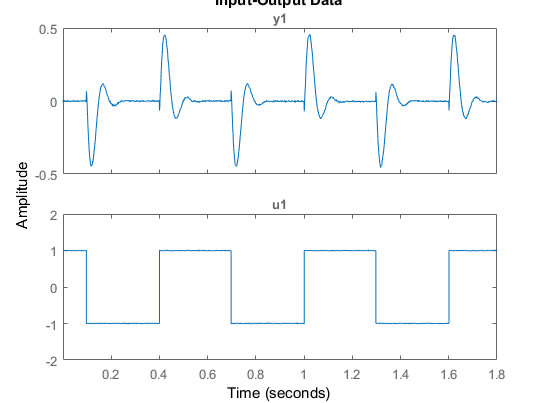
\includegraphics[width=0.5\textwidth]{Images/14.png}
\caption{ La réponse fréquentielle du filtre RII de type Chebychev 2 après l'amélioration des paramètres}
\end{figure}

\end{itemize}

\subsection{L'allure temporelle et le spectre d'amplitude de la gamme filtrée}

\label{matlab}
\lstinputlisting[caption = {Le script pur Tracer l'allure temporelle et le spectre d'amplitude de la gamme filtrée}]{8.m}

\begin{figure}[H]
\centering
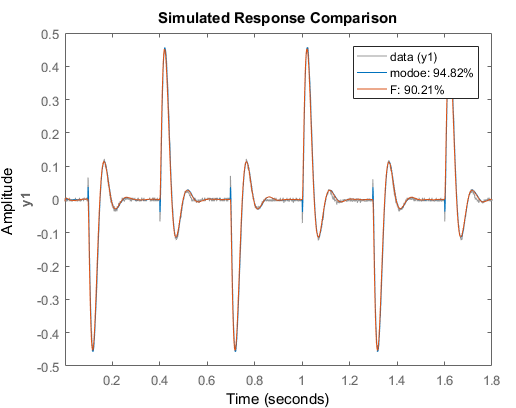
\includegraphics[width=0.5\textwidth]{Images/15.png}
\caption{ L'allure temporelle de la gamme filtrée}
\end{figure}

\begin{figure}[H]
\centering
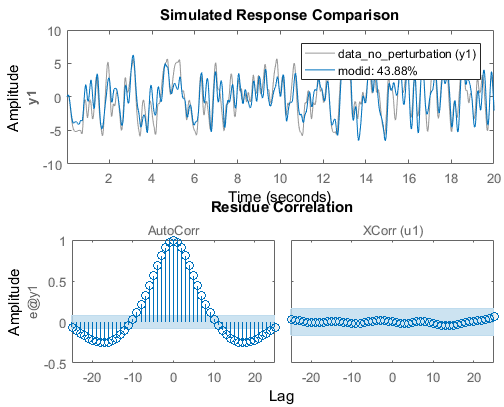
\includegraphics[width=0.5\textwidth]{Images/13.png}
\caption{ Le spectre d'amplitude la gamme filtrée}
\end{figure}

Cet résultat confirme les points remarqués sur le graphe de la réponse fréquentielle du filtre:
\begin{itemize}
\item
Le volume du son n'est pas altéré (sauf la note $Mi$), parce que le filtre ne présente pas des ondulations dans cette bande
\item La note $Fa$ qui correspond á la fréquence 349 est rejetée.
\item 
La note la plus proche $Mi$ est altéré par ce filtre. on peut régler ce problem en prenant les paramètres suivants:
$$\Delta f = 5$$
$$ f_c^b = 345 $$ 
$$ f_c^h = 345 $$ 
 On trouve le résultat désiré:

\begin{figure}[H]
\centering
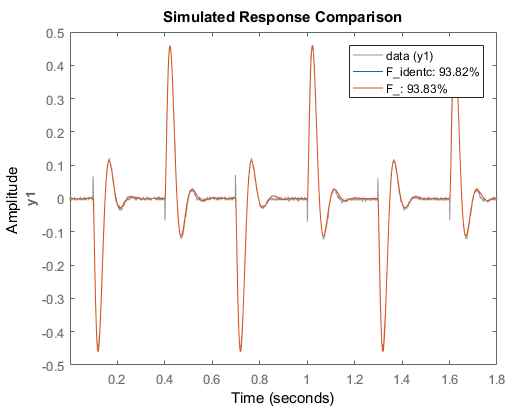
\includegraphics[width=0.5\textwidth]{Images/16.png}
\caption{ L'allure temporelle de la gamme filtrée après l'amélioration des paramètres}
\end{figure}

\begin{figure}[H]
\centering
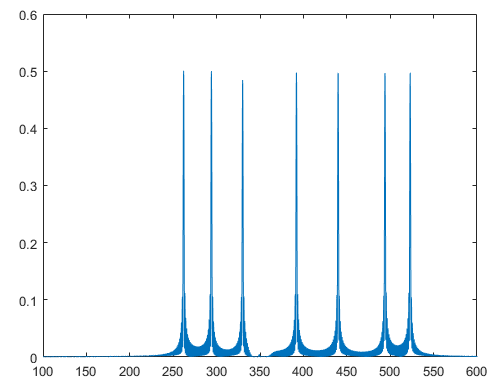
\includegraphics[width=0.5\textwidth]{Images/17.png}
\caption{ Le spectre d'amplitude de la gamme filtrée après l'amélioration des paramètres}
\end{figure}
\end{itemize} 
\newpage
\subsection{Le filtre RIF de longueur minimal (fenêtre de Kaiser)}

\label{matlab}
\lstinputlisting[caption = {Le script pur calculer Le filtre RIF de longueur minimal (fenêtre de Kaiser) et pour tracer la réponse fréquentielle et tracer la gamme filtrée}]{8.m}
 
 Les résultats de la simulation sont obtenus en utilisant les paramétrés suivants:
 $\Delta f = 5$, 
$ f_c^b = 345 $, et 
$ f_c^h = 345 $ \\
\begin{figure}[H]
\centering
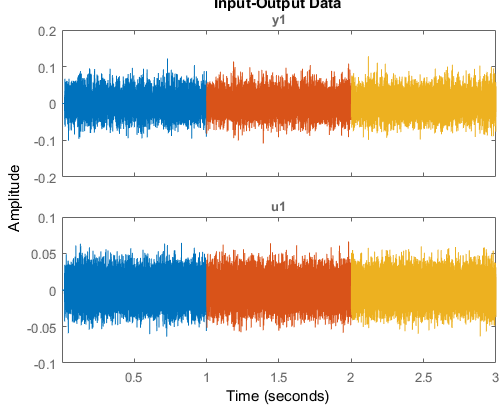
\includegraphics[width=0.5\textwidth]{Images/18.png}
\caption{ La réponse fréquentielle du filtre RIF ( avec fenêtre de Kaiser)}
\end{figure} 
 
\begin{figure}[H]
\centering
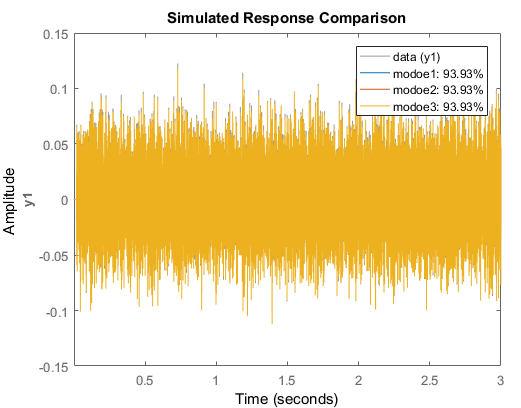
\includegraphics[width=0.5\textwidth]{Images/19.png}
\caption{ L'allure temporelle de la gamme filtrée }
\end{figure}

\begin{figure}[H]
\centering
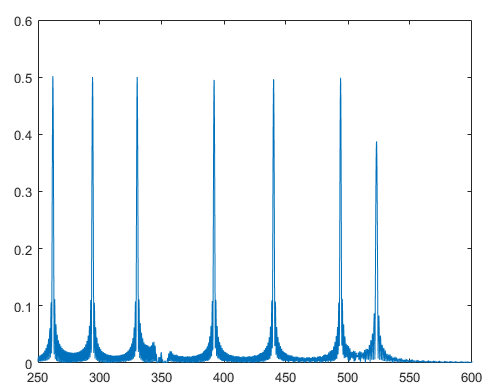
\includegraphics[width=0.5\textwidth]{Images/20.png}
\caption{ Le spectre d'amplitude de la gamme filtrée}
\end{figure}

\underline{Remarque}
Ce filtre a réalisé l'objective de la manière désirée.

\subsection{Comparaison entre le filtre de Chebychev de type 2 et celui de la RIF avec la fenetre de Kaiser}
On trace les deux réponses fréquentielles dans le même graphe.
 
\begin{figure}[H]
\centering
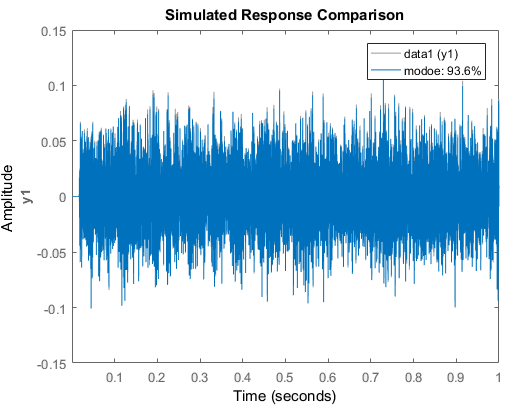
\includegraphics[width=0.5\textwidth]{Images/21.png}
\caption{ La réponse fréquentielle du filtre de Chebychev 2 et celui de la RIF ( avec fenêtre de Kaiser)}
\end{figure} 

\underline{Remarque}\\
Le graphe montre clairement que le filtre de RIF avec la fenêtre de Kaiser est plus performant que celui de Chebychev 2, en effet :
\begin{itemize}
\item
la bande á couper est plus courte que celle de Chebychev 2, que nous permet de remarquer le point suivant:
\item
Les informations utiles (les notes á conserver dans la bande passante) sont bien conservés, sans être influencée (le volume ne change pas).
\item
La coupure du filtre de RIF avec la fenêtre de Kaiser est plus raide que celle de Chebychev 2 (la bande de transition est très courte).
\end{itemize}

\subsubsection{Conclusion}
Le filtre de RIF avec la fenêtre de Kaiser est plus performant que celui de Chebychev 2.


\end{document}

